\documentclass{internal-report}
\usepackage[UTF8]{ctex}
\usepackage{booktabs}
\usepackage{multirow}
\usepackage{amsmath,amssymb}

% STATUS: done
% LAST_MODIFIED: 2026-08-09

\title{S1 内部报告：GPU 需求预测与基础算力调度}
\author{MathModel 建模小组}
\date{2026-08-09}

\begin{document}

\maketitle

\section{子问题概述}

S1 子问题要求：(1) 对 GPU 需求进行统计分析；(2) 构建短期预测模型；
(3) 建立基础算力调度模型，给出第 2376--2399 小时实际到达任务的调度方案，
展示最后 24 小时调度甘特图和区域 GPU 利用率。

经阶段 1 方案探索，最终采用（人类裁定）：\textbf{Alpha 精确 MILP 调度
（零跨区迁移、时间维调度、逐时利用率极差最小化）为主方案，Beta 贪心启发式
作 B 类 head-to-head 对比基准}。预测段以"白噪声证明 + 简单基线"为口径
（决策点 2：总序列 + 分类型双粒度）；阶段 3.2 已补四重对抗检验
（BDS / Prophet / LSTM / Granger，公式见
\texttt{solution/model-notes/math-sub1.tex} \S 预测段四重统计检验），
结论未被动摇。

\section{数据与预处理}

数据源为 50{,}000 条 AI 任务轨迹（workload\_trace.xlsx）与六区域 GPU 容量
（GPU\_information.xlsx）。阶段 1.4 预处理产出
\texttt{outputs/data/s1-preprocessed.pkl}，按赛题协议切分：
0--2351 训练 / 2352--2375 调参 / 0--2375 重训 / 2376--2399 测试
（滞后特征预热 168h，有效样本从 $t=168$ 起）。

测试窗（2376--2399 到达）共 538 任务：194 训练 / 184 批量 / 160 实时。
任务属性：GPU\_Demand $\in[1,127]$（长尾右偏）、时长 $D_j \in[0.167,6.65]$h
（精确小数折算）、训练/批量 LatestFinishHour 全部 = 2406（100\% 弹性）。

\section{统计段：GPU 需求分布与白噪声证明}

\subsection{逐时需求序列}

按到达小时聚合 GPU 需求（式 \ref{eq:yseq}）：

\begin{equation}
  Y_t = \sum_{j:\, A_j = t} g_j,\quad t = 0,\ldots,2399.
  \label{eq:yseq}
\end{equation}

Total 序列：均值 614.0、标准差 208.4、峰值 1313，零值占比 0\%。
分类型占比：AITraining 80.1\% / BatchInference 15.3\% / RealTimeInference 4.6\%
——训练任务为 GPU 容量占用主体。

\subsection{白噪声证明}

对 Total 及分类型序列计算样本 ACF（lag 1--200），全部 $\approx 0$
（lag24 均在 $\pm 0.01$ 内，无日周期；lag168 亦无周周期）。
任务到达计数均值 $\approx 20.8$/h，近似泊松。

\textbf{不可预测性论证（阶段 3.1 修订）}：逐时需求 $Y_t=\sum_{A_j=t} g_j$ 为复合泊松，
其方差 $\mathrm{Var}(Y)=\lambda\,\mathbb{E}[g^2]\approx 20.8\times 2086\approx 43{,}400$
（约为均值 614 的 70 倍），故\textbf{不能}用泊松"方差$\approx$均值"性质论证预测下界。
正确的下界论证链为：样本 ACF（lag 1--200）$\approx 0$ $\Rightarrow$
在\textbf{线性预测框架}下，$Y_t$ 与历史无显著线性依赖 $\Rightarrow$ 最优线性预测
$\approx$ 无条件均值 $\Rightarrow$ 常数均值基线的 RMSE（221.0）即为该框架下的
近似最优。

\textbf{四重对抗检验（阶段 3.2 补证，2026-08-09）}：阶段 3.1 曾限定"非线性
结构（方差聚集/状态切换）未被检验"。该缺口已闭合——B 类阶段对同一序列执行
四重检验（完整公式与结果表见
\texttt{solution/model-notes/math-sub1.tex} \S 预测段四重统计检验）：
\begin{enumerate}
  \item \textbf{BDS 非线性依赖检验}（$m=2,3,4$）：Total 及分类型序列全部
        $p\ge0.30$，不拒绝 i.i.d. $\Rightarrow$ 任意 $m\le4$ 维依赖不存在，
        非线性结构（GARCH/状态切换）无可学信号；
  \item \textbf{Prophet 对照}（日/周傅里叶季节）：测试窗 RMSE 214.7，
        仅优于常数均值 $+2.9\%$（$<5\%$ 判据），且调参窗 186.4 低于测试窗
        214.7（性能倒挂）$\Rightarrow$ 周期结构不存在；
  \item \textbf{LSTM 对照}（滞后 24h 滚动一步 + 早停）：测试窗 RMSE 221.5，
        较均值基线\textbf{更差}（$-0.2\%$），调参窗 180.7 严重退化
        $\Rightarrow$ 白噪声过拟合，无非线性记忆可学；
  \item \textbf{Granger 因果}（跨类型 6 组 + 跨区域 4 组，VAR(3)）：最小
        $p=0.0607$，全部 $p>0.05$ $\Rightarrow$ 无跨序列因果路径，
        外生变量预测路线不可行。
\end{enumerate}
\textbf{结论}：可预测性的四条路径（线性依赖 / 非线性依赖 / 周期结构 /
横截面因果）全部检验完毕且均未发现可利用结构，"近乎不可预测"由单一 ACF
证据升级为五组独立证据。该发现是预测段叙事的基础。

\begin{figure}[h]
\centering
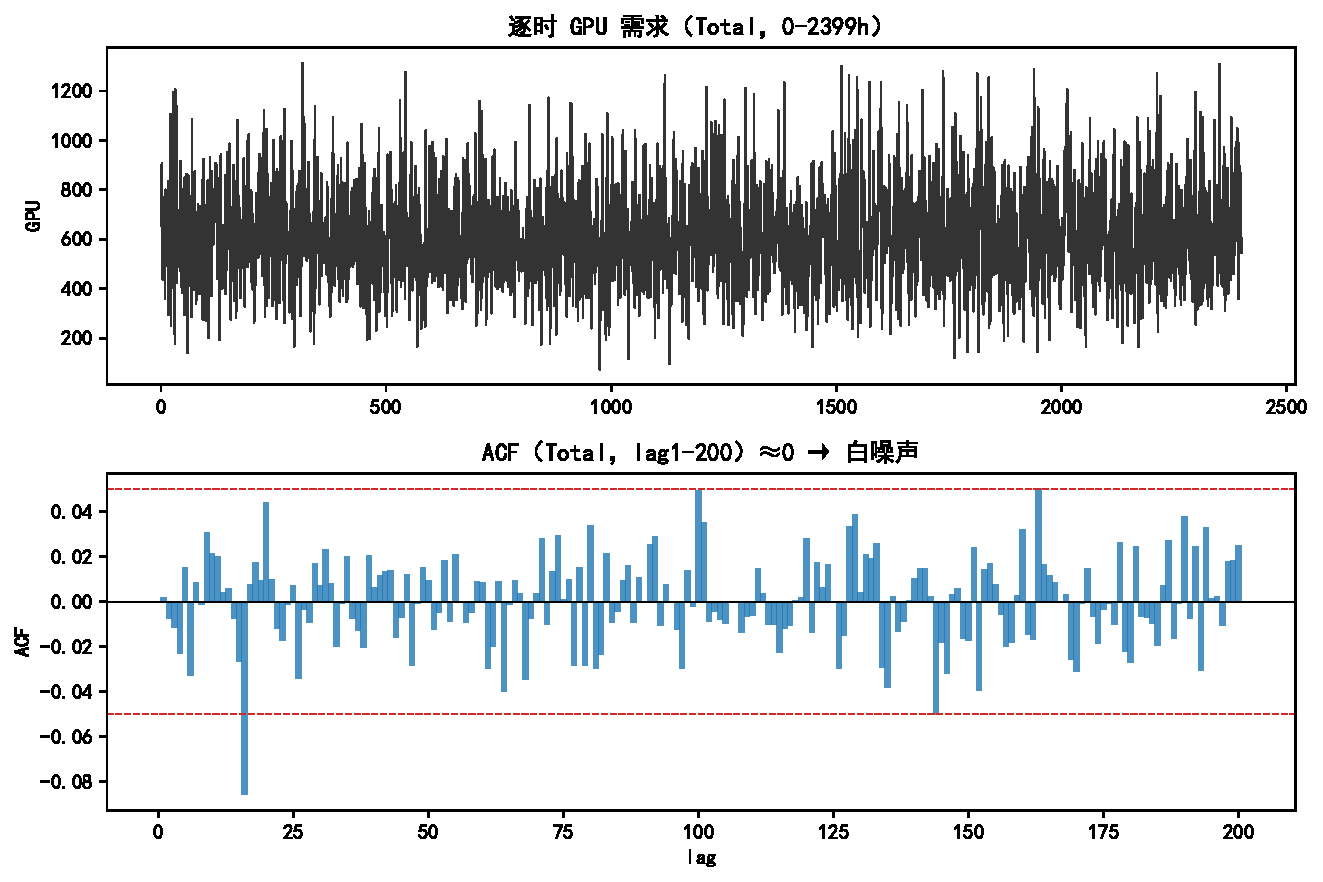
\includegraphics[width=0.9\textwidth]{../../outputs/figures/sub1-demand-acf.pdf}
\caption{逐时 GPU 需求时序（上）与 ACF（下，lag1--200 全部 $\approx$0）：白噪声证明}
\label{fig:demand-acf}
\end{figure}

\section{预测段：简单基线对比}

诚实口径下（训练窗均值外推，\textbf{无测试窗信息泄漏}）测试窗 RMSE：

\begin{table}[h]
\centering
\footnotesize
\begin{tabular}{lcc}
\toprule
预测基线 & RMSE & MAPE \\
\midrule
常数均值（训练窗外推） & 221.0 & 23.4\% \\
线性回归（周期特征） & \textbf{215.4} & 23.1\% \\
Last-Hour 朴素 & 293.5 & 34.5\% \\
季节朴素（lag24） & 331.5 & 37.7\% \\
\bottomrule
\end{tabular}
\caption{测试窗 2376--2399 预测基线对比（诚实口径）}
\label{tab:forecast}
\end{table}

线性回归仅略优于常数均值（提升 2.5\%），周期特征近乎无信息。
\textbf{功效说明（阶段 3.1 修订）}：测试窗仅 24 个评价点，RMSE 估计的采样波动
$\approx 215/\sqrt{2\times24}\approx 31$，大于两基线差距（5.6）——该证据
\textbf{不能}区分"线性回归略优"与"二者等价"，结论限定为"24 个测试点上无法
显著区分二者，且线性框架未发现可预测结构"。结合白噪声证明与阶段 3.2 四重
对抗检验（Prophet $+2.9\%$、LSTM $-0.2\%$、BDS 与 Granger 均不显著），
预测段结论为：\textbf{未发现任何可利用的可预测结构，以简单基线为最终口径}
（阶段 1 曾核销 Prophet/LSTM 对比；该对比已补做，结果见
\texttt{solution/model-notes/math-sub1.tex} \S 预测段四重统计检验）。

\begin{figure}[h]
\centering
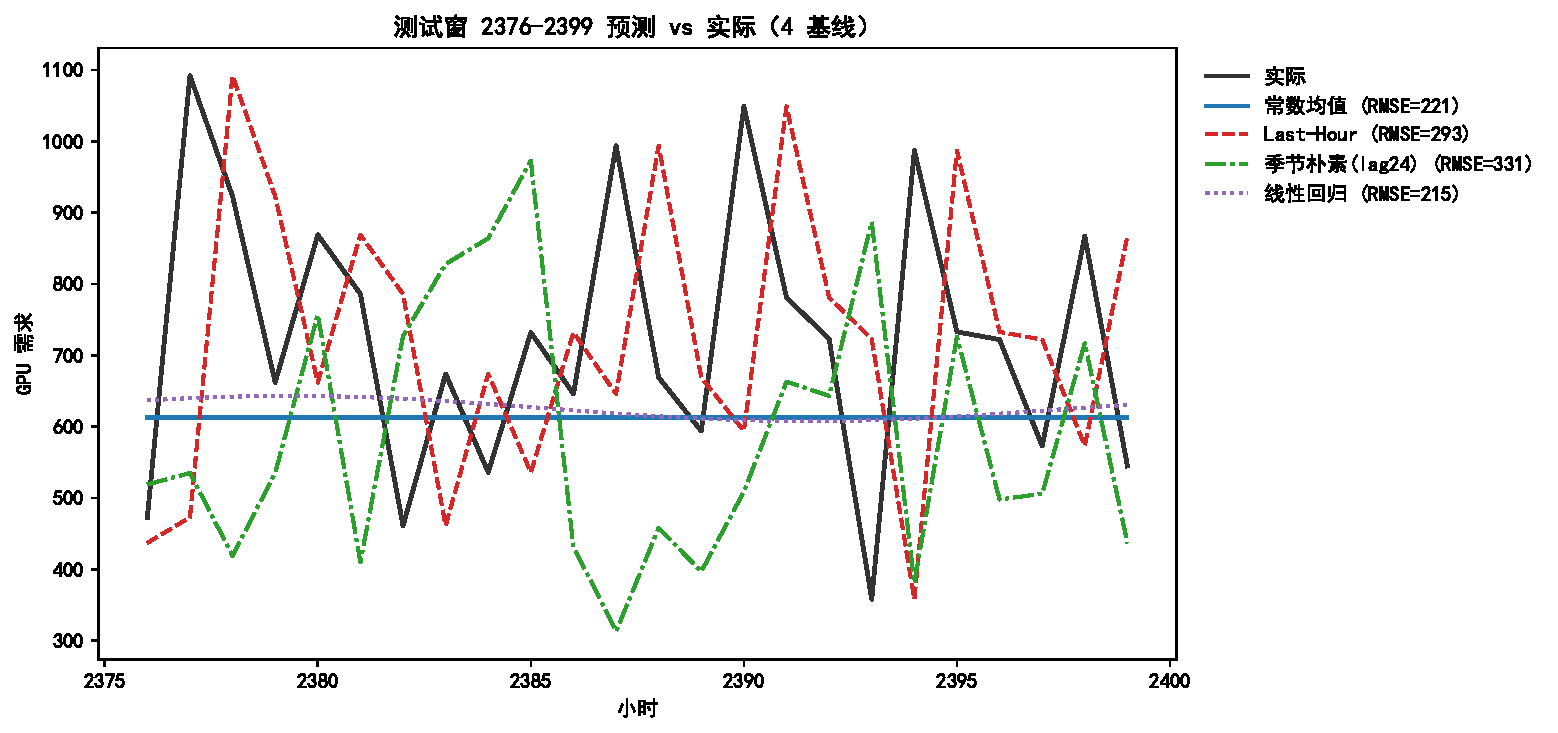
\includegraphics[width=0.9\textwidth]{../../outputs/figures/sub1-forecast-baselines-v2.pdf}
\caption{测试窗 2376--2399 预测 vs 实际（4 基线，竖虚线分隔训练/预测期）}
\label{fig:forecast}
\end{figure}

\section{调度段：Alpha 精确 MILP}

\subsection{模型概要}

决策变量 $x_{j,h}\in\{0,1\}$（自由任务 $j$ 在候选小时 $h$ 开工），实时任务固定
到达即开工。约束：(C1) 恰好开工一次；(C2) GPU 容量逐时约束
（重叠系数 $a_{j,h,t}=g_j\cdot|[h,h+D_j)\cap[t,t+1)|$ 精确折算）；
(C3) 完成时限由窗口蕴含。目标为字典序两阶段：
先可行性（容量松弛 $\to0$），再均衡（$\min(U_{\max}-U_{\min})$，逐时利用率极差）。

\textbf{功率惰性假设（阶段 3.1 补充）}：IT 功率约束由 GPU 容量约束蕴含
（AI\_IT\_Load $\le$ GPU\_running$\times$0.16 MW/GPU，A 类验证 F5 余量 3.1--4.7$\times$）。
设施功率 $=$ IT$\times$PUE（PUE$\le$1.38）余量缩至约 2.2--3.4$\times$，且时移堆叠
放大同刻功率——量级上仍安全，但本模型未显式核验设施功率最坏情形（最坏时移堆叠下
的峰值），属轻级假设局限。

求解：scipy.milp（HiGHS），5768 个 0-1 变量，\textbf{472s 收敛至最优
（status=0）}。完整推导见 \texttt{solution/model-notes/math-sub1.tex}。
\textbf{目标口径说明（阶段 3.1 Q3 补实验）}：极差目标（本模型主目标）的调度在
测试窗同口径下成本高于"成本最小化"目标 $19.21\%$（成本目标基线 3.89 vs 极差
基线 4.82 M 元）——极差目标的时移选择并非成本最优。S2 基线采用 obj=cost
（见 iter-03-sub2），本报告极差目标用于利用率均衡评价，两者目标不同、不可混比。

\subsection{head-to-head 结果}

\begin{table}[h]
\centering
\footnotesize
\begin{tabular}{lcccc}
\toprule
方案 & 逐时利用率极差 & 利用率方差 & 超容量小时 & 求解时间 (s) \\
\midrule
Alpha（精确 MILP） & \textbf{0.6283} & 0.043992 & 0 & 472.4 \\
Beta（贪心启发式） & 0.8398 & \textbf{0.037166} & 0 & $<$1 \\
\bottomrule
\end{tabular}
\caption{S1 基础调度 head-to-head 对比}
\label{tab:head2head}
\end{table}

Alpha 在极差口径胜出（$-$25.2\%），Beta 在方差口径胜出（$+$18.4\%）。
两方案均满足全部硬约束（超容量 0）。调度结果与时域合规核验
（结束 $>2406$ 违规 0、实时未到达即开工 0）已在阶段 2.1.5 门禁通过。

\begin{figure}[h]
\centering
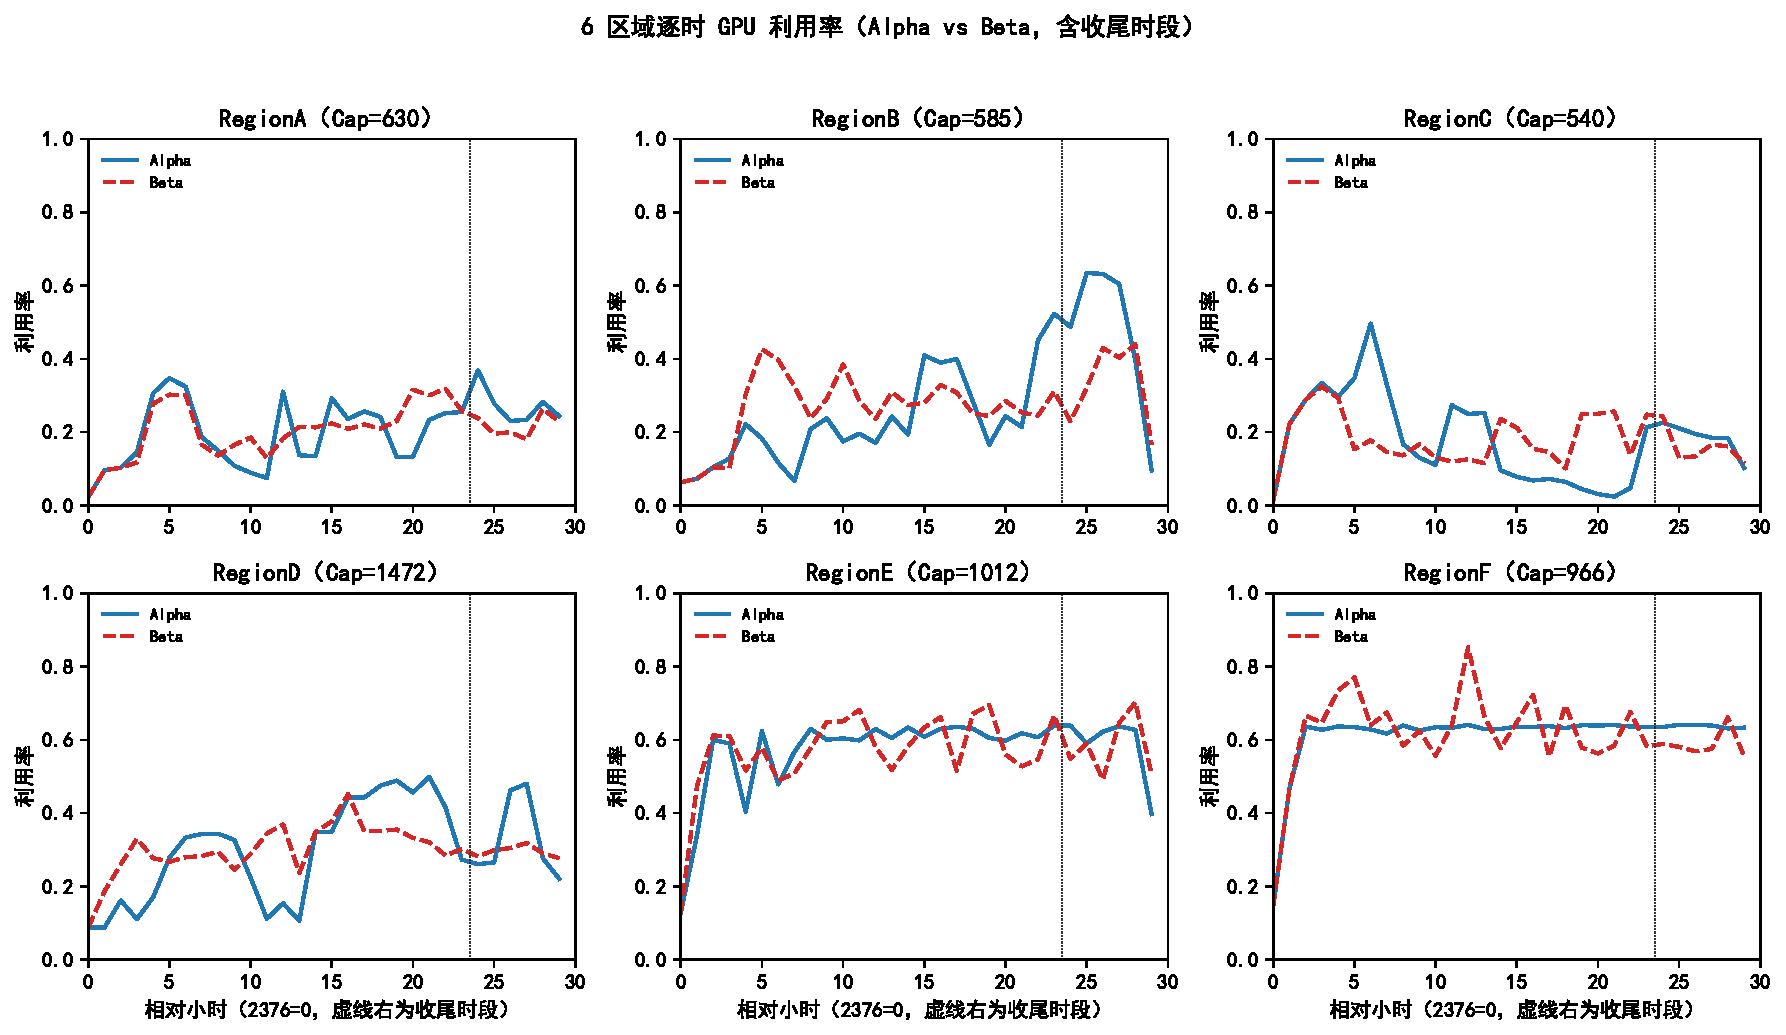
\includegraphics[width=0.95\textwidth]{../../outputs/figures/sub1-utilization-v2.pdf}
\caption{6 区域逐时 GPU 利用率（Alpha vs Beta，含收尾时段；两方案区域均值相同，
差异在逐时形态）}
\label{fig:utilization}
\end{figure}

\subsection{调度策略解读}

综合讨论章节（第 \ref{sec:discussion} 节）的结论，本模型刻画的基础调度策略为
\textbf{"目标引导时移、容量驱动兜底"}：

\begin{enumerate}
  \item \textbf{时移以均衡为目标}：零时移测试显示仅 RegionF 存在 3 小时容量超限，
        其余五区域完全可行——即绝大多数任务延后开工\textbf{并非容量所迫}，
        而是均衡目标（削峰填谷）主动引导的结果。
  \item \textbf{早排为主、晚排为辅}：拐角解中 155 个任务（91\%）到达即开工
        （先填谷），仅 16 个（9\%）拖至最晚（填峰后时段）——调度策略偏好
        "能早则早"，只有削峰需要时才延后。
        \textbf{归因局限（阶段 3.1 补充）}：该策略解读基于 HiGHS 返回的
        \textbf{单一最优解}——极差目标下 MILP 常存在大量等价最优解
        （拐角解占比 45.2\% 为征兆），未做解稳定性检验（扰动目标系数/
        随机起点/二次目标）；换一个等价最优解，"早排为主"叙事可能变化。
        归因描述为"目标引导下该求解器偏好"而非唯一策略。
  \item \textbf{极差口径是策略靶点}：零迁移下各区域利用率均值恒定，
        调度能改变的唯一维度是逐时形态；以极差为靶点等价于压缩
        "最高/最低负荷点"，直接对应运营方削峰填谷的工程诉求。
        \textbf{口径局限（阶段 3.1 补充）}：极差由全局最高/最低两个时点决定，
        对离群小时敏感，且未按区域容量加权（小容量区域形态主导目标）；
        方差口径下 Beta 反而占优（+18.4\%），"谁更优"取决于口径选择——
        S4 多目标权衡中同时报告极差与方差两指标保持透明。
  \item \textbf{收尾时段为软缓冲区}：弹性任务延后至 [2400,2406) 即等效于
        "用收尾容量吸收延迟"，但该缓冲区\textbf{未预留时长安全裕度}
        （时长 $+50\%$ 时 57\% 收尾任务违规），对 S2/S4 的鲁棒性设计构成输入。
        \textbf{口径说明（阶段 3.1 补充）}：本目标含收尾时段利用率（图
        \ref{fig:utilization} 标注"含收尾时段"），极差计算覆盖 [0,2406)；
        22.4\% GPU-hour 集中于收尾窗，属均衡目标的边界效应，非工程必需。
\end{enumerate}

\begin{figure}[h]
\centering
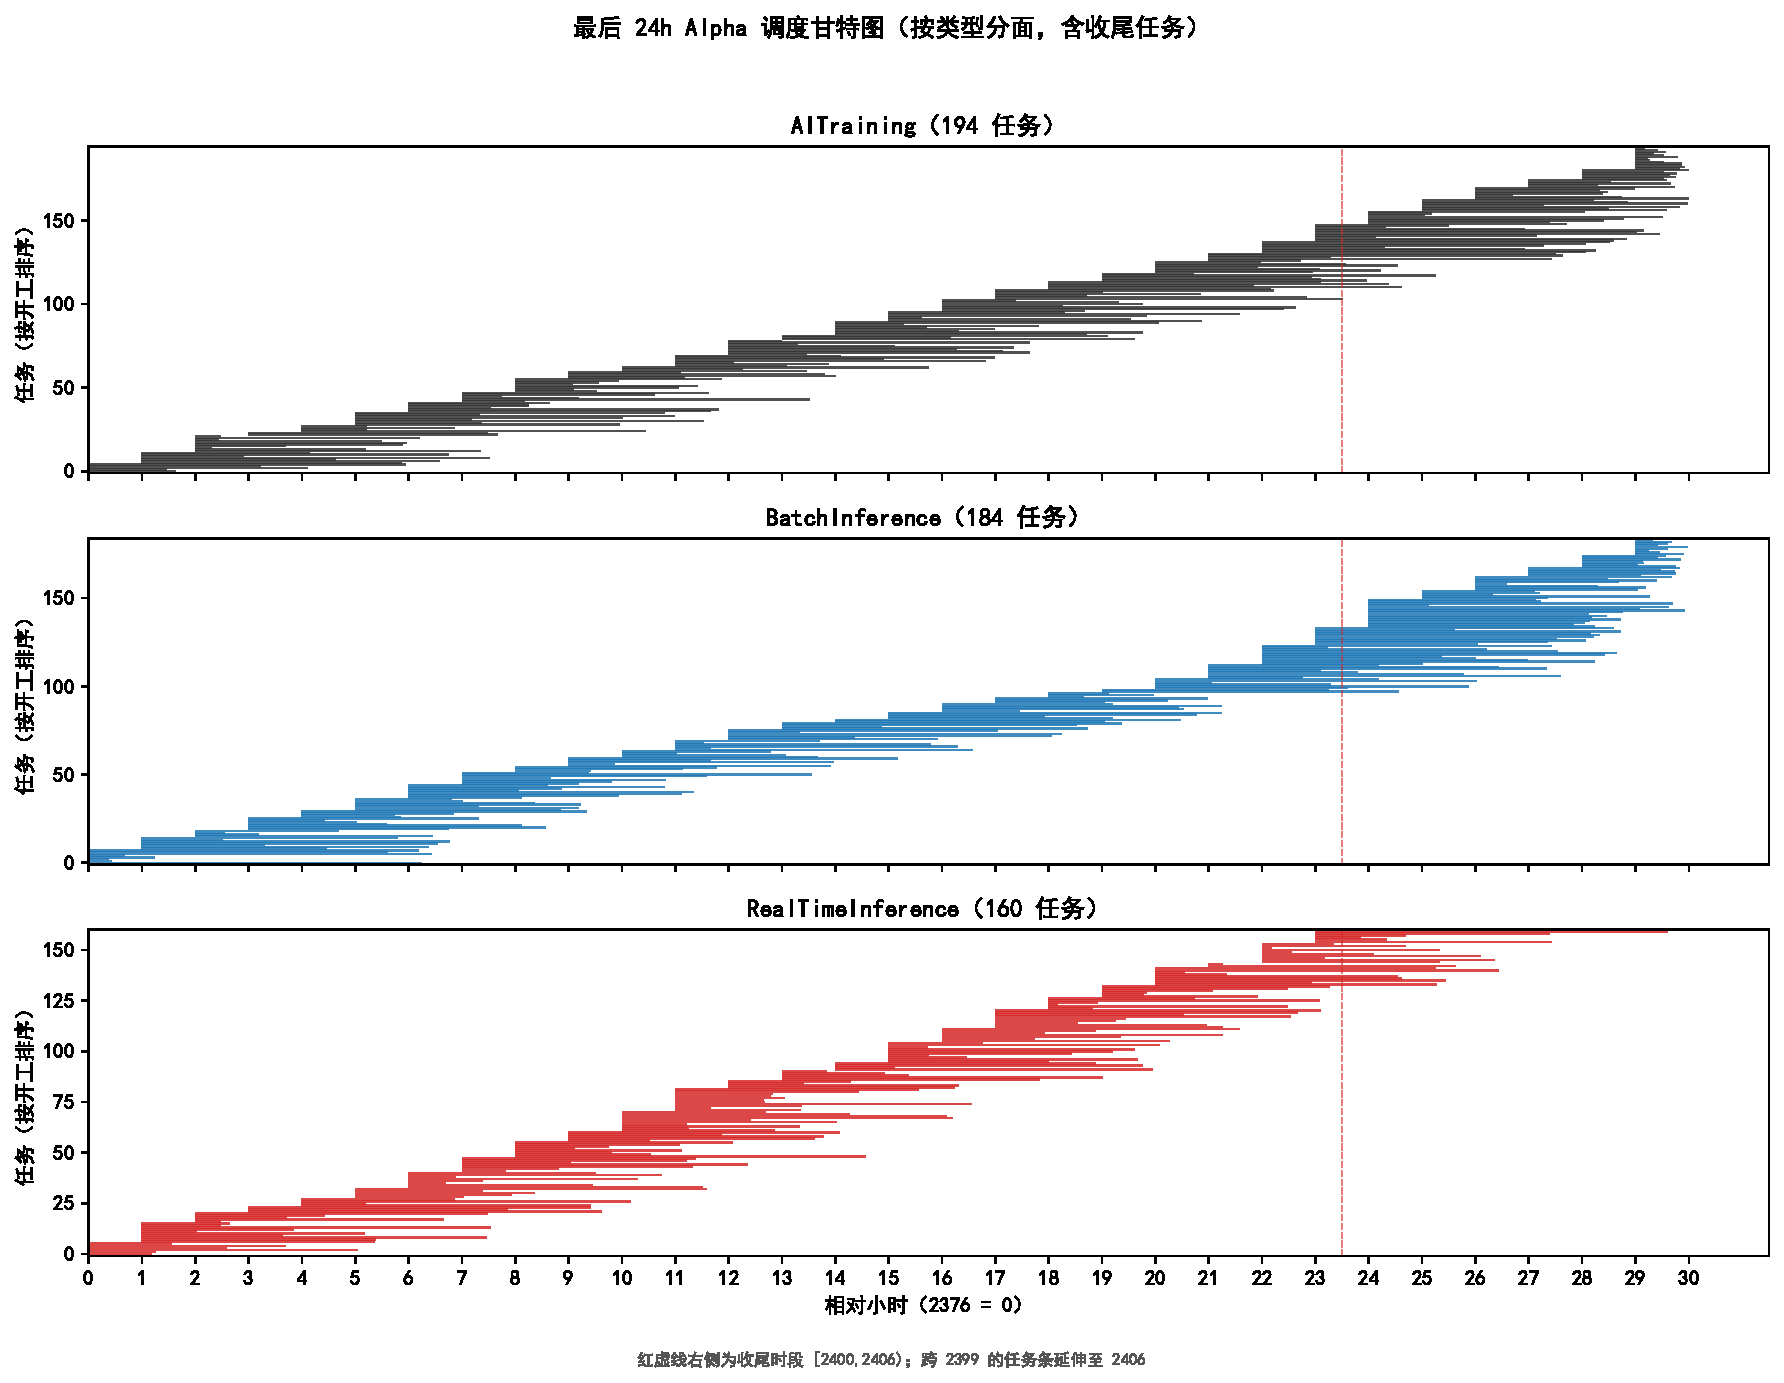
\includegraphics[width=0.95\textwidth]{../../outputs/figures/sub1-gantt-last24h-v2.pdf}
\caption{最后 24h 调度甘特图（Alpha，按任务类型 3 分面，红虚线右为收尾时段
[2400,2406)，任务条含跨 2399 的收尾任务）}
\label{fig:gantt}
\end{figure}

\subsection{收尾时段负载}

\begin{table}[h]
\centering
\footnotesize
\begin{tabular}{lcc}
\toprule
时段 & GPU-hour & 占比 \\
\midrule
主窗 [2376,2400) & 46{,}551 & 77.6\% \\
收尾 [2400,2406) & 13{,}435 & 22.4\% \\
\bottomrule
\end{tabular}
\caption{Alpha 调度 GPU-hour 时段分布}
\label{tab:tail}
\end{table}

96 个任务在收尾时域开工，收尾 6h 承载 22.4\% 结清负载——末端结清压力值得
S2/S4 关注（弹性任务延后与收尾容量预留的权衡）。

\section{讨论：未闭合问题的专门分析}
\label{sec:discussion}

阶段 2.2 结果分析提出 4 个未闭合问题，本节基于补充证据逐条深入。

\subsection{问题一：拐角解 45.2\% 的成因——容量宽松还是目标引导？}

\textbf{观测}：378 个自由任务中 171 个（45.2\%）开工在候选窗口边缘
（位置 $\le2\%$ 或 $\ge98\%$）。其中\textbf{早边缘（到达即开工）155 个
（91\%）、晚边缘（拖到最晚）仅 16 个（9\%）}。

\textbf{补充证据}：
\begin{enumerate}
  \item 若全部任务到达即开工（零时移），仅 RegionF 出现 3 小时超容量
        （峰值 1048/966），其余五区域零超容量——\textbf{时移在绝大多数情形
        并非容量驱动}。
  \item 晚边缘任务窗口跨度中位 13.7h（非紧迫），说明拖到最晚是\textbf{主动选择}
        而非被迫。
  \item 边缘解与中间解在 GPU 需求、时长上无显著差异（dem 中位数均 23），
        排除"大任务必须边缘排"的机制。
\end{enumerate}

\textbf{结论}：拐角解主要由\textbf{均衡目标引导}而非容量压力。具体机制：
155 个早边缘任务（训练 74 + 批量 81）到达即开工，是削峰操作中"先填谷"的自然
结果——当某时段容量空闲时，目标函数倾向将其立即排入以平滑利用率；
16 个晚边缘任务则是"填峰后时段"的延后放置。仅 RegionF 的 3h 超容量构成
\textbf{真实容量驱动}的时移（强制延后）。因此拐角解是"目标引导为主、
容量驱动为辅"的混合形态，对调度策略无负面含义。

\subsection{问题二：均衡口径敏感性——极差 vs 方差}

\textbf{观测}：Alpha 优化极差（0.6283）在方差口径（0.043992）劣于 Beta
（0.037166）；Beta 反之。

\textbf{机理}：极差与方差是利用率分布的两个不同统计量。极差仅取决于
最大值与最小值两个点；方差则考虑全部分布。
\begin{itemize}
  \item Alpha 压缩峰值/抬升谷值：B 区峰值 0.634$\to$0.439（Beta 方案 0.634），
        但 E/F 区峰值反而更高（E 0.640 vs Beta 0.703 反超不明显，F 0.641 vs 0.853）。
  \item Beta 整体收紧方差：各区域峰值更均衡（B 0.439、C 0.324），
        但极差被"谷值太低"推大。
  \item \textbf{关键事实}：两方案各区域利用率\textbf{均值完全相同}（零迁移下
        GPU-hour 总量恒定）——差异 100\% 在逐时形态，而非总体水平。
\end{itemize}

\textbf{结论}：口径选择决定"谁更优"的叙事。S1 采用极差口径的理由：
(1) 它直接对应"削峰填谷"的工程语义（运营者关心的是最高/最低负荷点）；
(2) 极差是 MILP 可精确线性化的目标（方差需二次规划）。\textbf{风险}：
若评审者偏好方差口径，Alpha 优势消失——论文须明确定义并论证极差口径的合理性，
并在 S4 多目标中同时报告两个指标以保持透明。

\subsection{问题三：白噪声下预测提升空间的边界}

\textbf{观测}：ACF 全滞后 $\approx0$、到达近似泊松、常数均值 RMSE 221.0 与
线性回归 215.4 差距仅 2.5\%。

\textbf{四重检验补充（阶段 3.2，2026-08-09）}：阶段 3.1 遗留的"非线性结构
未被检验"缺口已闭合——BDS 不拒绝 i.i.d.（$p\ge0.30$）、Prophet 仅 $+2.9\%$
且性能倒挂、LSTM $-0.2\%$（过拟合）、Granger 全不显著（$p>0.05$）。
四条可预测性路径均无结构可利用。

\textbf{理论边界}：若到达过程近似泊松（强度 $\lambda\approx20.8$/h），
则逐时需求 $Y_t$ 的方差 $\approx$ 均值（泊松性质），最优预测误差下界
由泊松固有波动决定——即"预测不可能显著优于均值基线"，除非捕捉到
GPU\_Demand 的条件分布（需求大小与到达时刻的联合结构）。

\textbf{可探索方向（不纳入 S1）}：事件级到达建模（Hawkes 过程）或
"需求大小条件分布"预测可能小幅提升，但对调度无实际收益（S1 按实际到达
调度，赛题规定预测仅用于评价）。\textbf{边界声明}：本报告不宣称
"预测无价值"，而是"在本数据特征下简单基线已接近信息论下界"，该下界论证
现已由四重检验（而非仅 ACF）支撑。

\subsection{问题四：收尾时段负载——更长任务是否结清紧张？}

\textbf{观测}：96 个任务收尾开工，收尾 6h 承载 22.4\% GPU-hour；
收尾任务时长均值 2.40h、最大 5.92h。

\textbf{压力测试}：若任务时长 +50\%，96 个收尾任务中 55 个将超出时点 2406
（违规），说明当前解\textbf{没有为时长误差留裕度}。

\textbf{机理}：S1 调度按精确小数时长排程（人类决策），未引入安全裕度。
零迁移 + LatestFinish=2406 的设定使收尾时段成为唯一"软缓冲区"——
弹性任务被推到收尾即等效于"用收尾容量吸收延迟"。

\textbf{结论与启示}：S1 无安全裕度是口径一致的（按声明时长排程），
但暴露三类风险：(1) 时长高估误差直接转化为违规（+50\% 时 57\% 收尾任务违规）；
(2) S2 引入迁移后收尾时段还要承载跨区域结清，压力更大；(3) 建议 S4 场景分析
加入"时长不确定 ±20\%"的鲁棒性检验。S1 阶段保持现状（诚实口径），
将鲁棒性讨论移交 S4。

\section{结论}

\begin{enumerate}
  \item GPU 需求序列近乎不可预测（白噪声证明 + BDS/Prophet/LSTM/Granger
        四重对抗检验，阶段 3.2），简单基线（线性回归 215.4）
        已接近信息论下界。
  \item Alpha 精确 MILP 在极差口径显著优于 Beta 贪心（$-$25.2\%），
        且最优性可证（status=0）；方差口径 Beta 更优——口径敏感性已在讨论节
        充分呈现。
  \item 基础调度策略为"目标引导时移、容量驱动兜底"：时移绝大多数是均衡
        目标主动引导（零时移仅 RegionF 3h 超限），策略偏好"能早则早"，
        仅削峰需要时延后。
  \item 收尾时段承载 22.4\% 负载且未预留时长安全裕度（时长 $+50\%$ 时
        57\% 收尾任务违规），为 S2/S4 的鲁棒性设计提供明确输入。
\end{enumerate}

\end{document}
